\section{Umsetzung}
Für die Umsetzung wurde ein Android-Smartphone, ein Lenovo K6 mit einem Qualcomm Snapdragon 430 Prozessor \cite{qualcomm} verwendet.
Hingegen zu älteren Smartphones unterstützen Neuere den USB On-The-Go (OTG) Modus, womit die Stromversorgung des Arduinos über USB-Anschluss gewährleistet wird.

Desweiteren wurde ein Arduino CH340 chip verwendet und als Beschleunigungssensoren das Modell MPU-6050.
Zur Kommunikation mit dem Arduino und abgreifen der Beschleunigungssensoren des Sensors wurden die Bibliotheken \textit{usb-serial-for-android} \cite{mik3y} und \textit{UsbSerial} \cite{felHR85} verwendet.

Die synthetisch erzeugten Schlagzeuggeräusche für Hihat, Snare und Bass wurden synthetisch mit PureData \cite{puredata} erzeugt. 
Zur Nutzung der PureData-Patches auf dem Android Gerät, wurde die Bibliothek \textit{pd-for-android} \cite{pdAndroid} von \textit{libpd} verwendet.
Diese unterstützt keine erweiterten Funktionen, wie sie in PureData Extended vorkommen.

Die Android-App wurde in Java geschrieben und unter der Laufzeitumgebung Android-Version 7.0 getestet.
Abbildung \ref{fig:app} zeigt den Aufbau der Anwendung mit dem Arduino und den beiden MPU-6050 Sensoren.
Die Sensoren werden bei Testzwecken am jeweiligen Objekt fixiert, so dass die Y-Achse des Beschleunigungssensors nach oben zeigt.


\begin{figure}[H]
	\centering
	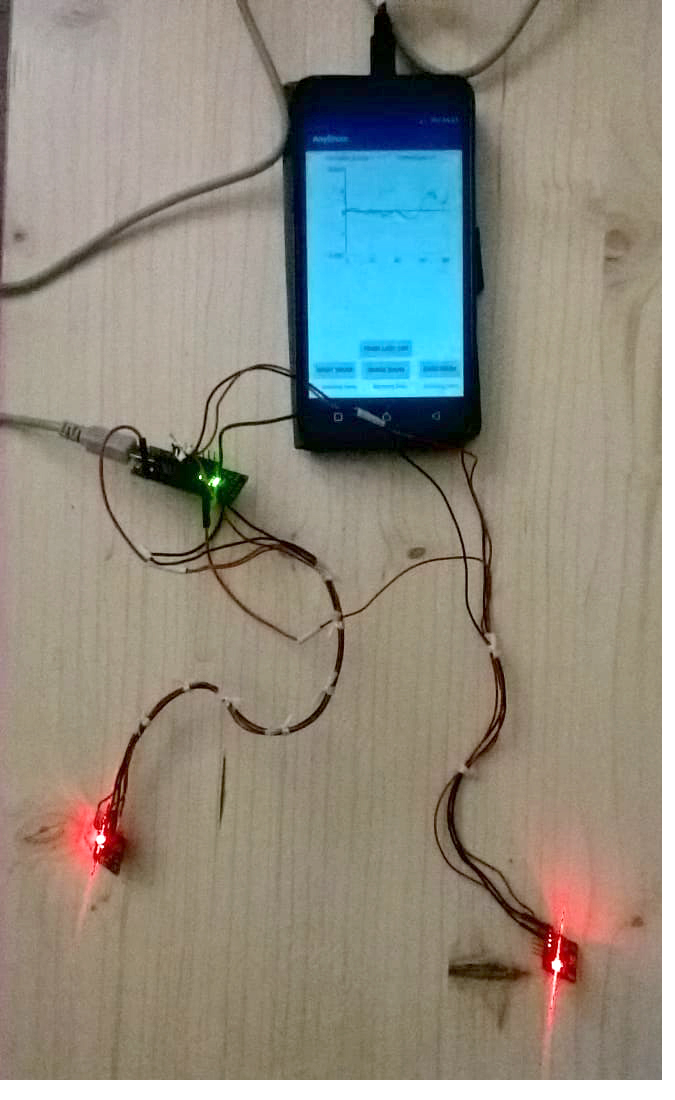
\includegraphics[scale=0.25]{figures/aufbau.jpg}
	\caption{Aufbau mit Arduino auf Holzplatte}
	\label{fig:app}
\end{figure}

